\section{\texorpdfstring{Seiduv switching}{Seiduv switching}}

\vspace{5mm}
\large


\begin{definition}
Necht V je V.P nad T. Linearni forma je lin zobrazeni $f:V \to T$. Pak linearni formy tvori V.P. nad T. Znacime $V^{\ast}$ a je tzv. dualni prostor k V.
\end{definition}
\begin{definition}
Necht $B = \{b_1, b_2, ..., b_n\}$ je baze V, pak $B^{\ast} = \{ f_1, f_2, ..., f_n \}$ je dualni baze, pokud formy jsou dane predpisem:
\[ f_i(b_j)= \twopartdef{1}{i = j}{0}{jinak} \]
\end{definition}
\begin{definition}
Necht A,B jsou V.P nad T, $dimA = n, dimB = k$. Necht $\varphi:A \to B$ homomorf. Pak dualni homomorf k $\varphi$ je zobrazeni $\varphi^{\ast}: B^{\ast} \to A^{\ast}$ dane predpisem:
\[ \forall f \in B^{\ast}\  \forall u \in A: (\varphi^{\ast}(f))(u) = f(\varphi(u)) \]
\end{definition}


\begin{theorem}[Matice dualniho homomorf(BD)]
Matice dualniho homomorf vzhledem k dualnim bazim je transponovanout matici k matici primarniho homomorf.
\[ \prescript{}{C^{\ast}}{[\varphi^{\ast}]}_{B^{\ast}} = (\prescript{}{B}{[\varphi]}_{C})^T \]
\end{theorem}
\begin{proof}
	Matice zobrazeni linearni formy z prostoru $f:V \to T$ je
	\[ \prescript{}{B}{[f]}_{k} = (f(b_1), f(b_2),...,f(b_n)) \]

	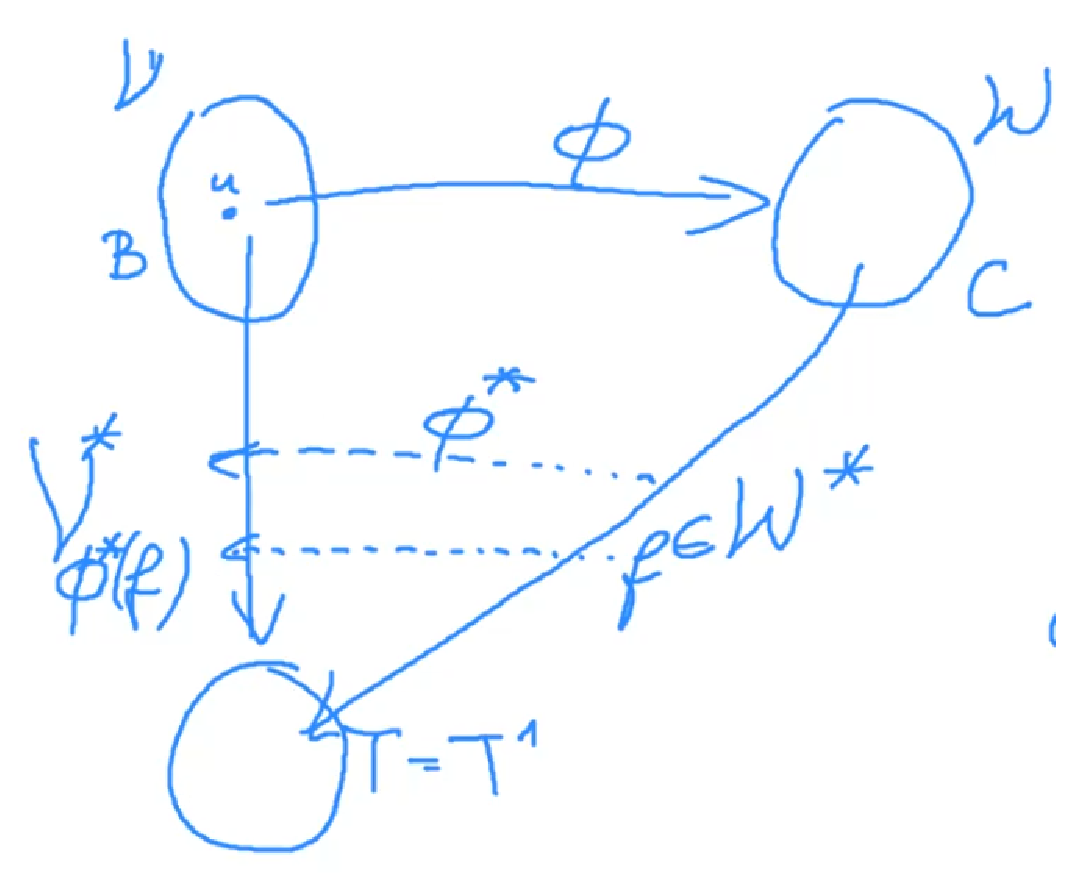
\includegraphics[scale=0.4]{dual_1.eps}

	Mame homomorf $\phi:V \to W$, pak linearni formy $h:W \to T$.

	Dualni homomorf $\phi^{\ast}:W^{\ast} \to V^{\ast}$ je definovan:
	\[ \phi^{\ast}(f)(u) = f(\phi(u)) \]

	Jelikoz lin formy jsou n-tice, tak $dim(V) = dim(V^{\ast})$.

	Matice $\phi$ je $\prescript{}{B}{[\phi]}_{C} \in T^{k \times n}$.
	Matice $\phi^{\ast}$ je $\prescript{}{C^{\ast}}{[\phi^{\ast}]}_{B^{\ast}} \in T^{n \times k}$.

	Veta rika, ze
	\[ \prescript{}{C^{\ast}}{[\varphi^{\ast}]}_{B^{\ast}} = (\prescript{}{B}{[\varphi]}_{C})^T \]
\end{proof}

\begin{definition}
Faktorprostor: faktorizace dle podprostoru W prostoru V (podgrupa). $V/W$ jsou mnoziny $\forall u \in V u + W$. Pak i faktorprostor je V.P vuci operacim:
\[ (u + W) + (a + W) = (u + a)W, \lambda cdot (u + W) = (\lambda \cdot u) + W \]
Plati: $dim(V/W) = dimV - dim W$.
\end{definition}

\begin{theorem}[Izomorfismus faktorprostoru]
	Necht $V = T^n$ a necht W je podprostor. Pak
	\[ V/W^{\perp} \sim W^{\ast} \]
\end{theorem}
\begin{proof}
	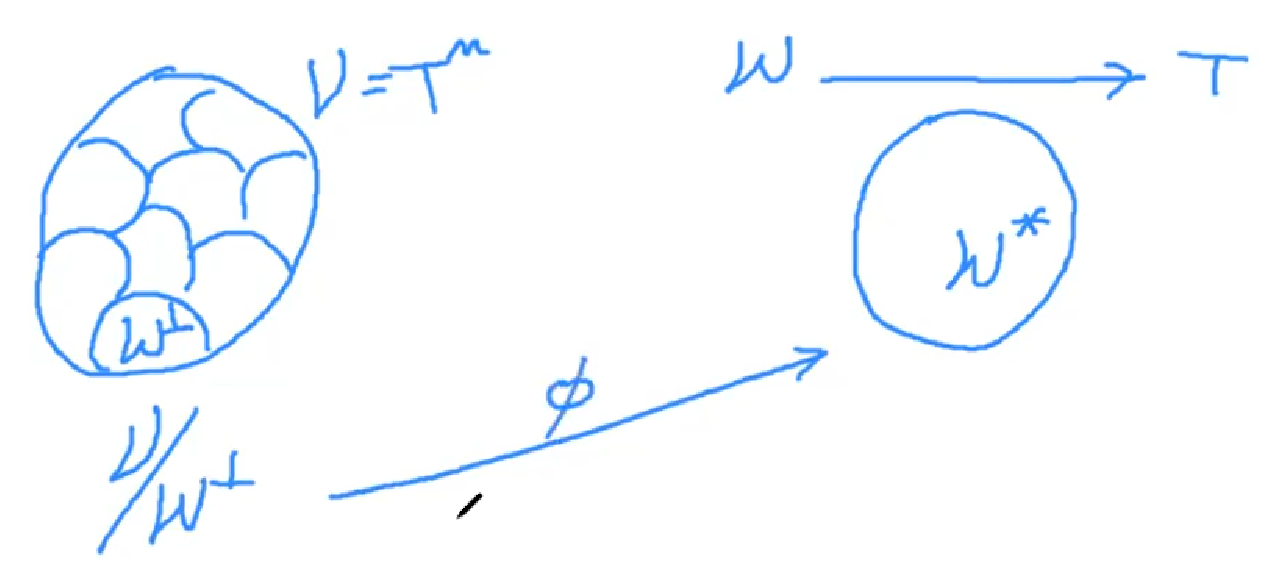
\includegraphics[scale=0.4]{dual_2.eps}

	Pak izomorf $\phi$ je definovan:
	\[\phi(v + W^{\perp} = \langle v, \cdot \rangle \]
	Udelali jsme linearni formu z bilinearni??

	Pokud dosadime promennou:
	\[\forall x \in W: \phi(v + W^{\perp})(x) = \langle v, x \rangle \]

	Chceme aby $\phi$ bylo korektne definove a splnovalo vlastnosti izomorf:

	1) korektnost definice \\
	2) lin zobrazeni \\
	3) proste\\
	4) na

	Dukaz:\\
	1) $a \in v + W^{\perp} \iff a = v + b, b \in W^{\perp}$. Pak
	\[ \langle a, x \rangle = \langle v + b, x \rangle = \langle v, x \rangle + \langle b, x \rangle\]
	Protoze $x \in W \Rightarrow \langle b, x \rangle = 0 \Rightarrow \langle v, x \rangle = \langle a, x \rangle $.

	2) Skalarni soucin je bilinearni forma, z toho $\phi$ je linearni zobrazeni.\\
	3) Necht $\phi(v + W^{\perp}) = 0 \Rightarrow \forall x \in W : \langle v, x \rangle = 0 \Rightarrow v \in W^{\perp} \Rightarrow v + W^{\perp} = \bar{0} + W^{\perp}$.
	Takze v kernelu je pouze $W^{\perp}$.

	4) Nahledneme z dimenzi.
	\[ Im(\phi) \leq W^{\ast} \land dim(Im(\phi)) = dim (V/W^{\perp}) \]
	Rovnost dimenzi plati protoze zobrazeni je proste.
	\[ dim(Im(\phi)) = dim(V) - dim(W^{\perp}) = dim(V) - (dim(V) - dim(W)) = dim(W) = dim(W^{\perp}) \]

	Z LA $Im(\phi)$ je vnoreny podpostor stejne dimenzi jako nadprostor $\Rightarrow$ jsou stejne.

\end{proof}

\begin{theorem}[Burnsidovo lemma(BD)]
\end{theorem}

\begin{lemma}
Necht grupa $G$ provadi akci na mnozine $M$, grupa $H$ na $N$. Necht $\varphi:M \to N$ bijekce.
	\[ if g \in G, h \in H, \forall m \in M: h\varphi(m) = \varphi(gm) \Rightarrow |G_{g}| = |H_{h}| \]

	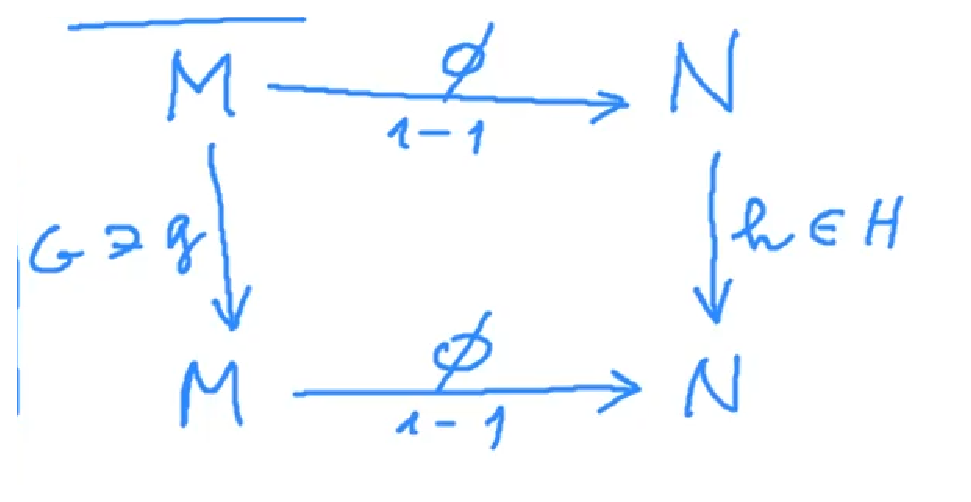
\includegraphics[scale=0.4]{group_lemma.eps}
\end{lemma}
\begin{proof}
Prvky v $M_g$ jsou $gm = m$. Prvky v $N_h$ jsou $hn = n$. Kvuli bijekci n lze jednoznacne vyjadrit jako:
\[ n = \varphi(m) = \varphi(\varphi^{-1}(n)) \]
Pak
\[ h\varphi(m) = \varphi(m) \]
Diagram komutuje
\[ \varphi(gm) = \varphi(m) \]
$\varphi$ je bijekce, takze proste $\Rightarrow gm = m$. Dohromady \# $hn = n$ je totez jako \# $gm = m$.
\end{proof}

\begin{definition}
Seiduv switching vymeni vsechny hrany a nehrany vychazejici z $u \in V$. Ostatni vrcholy a hrany beze zmen. Grafy $G \sim G' \iff G'$ lze ziskat z G postupnym prepinanim vrholu.
\end{definition}

\begin{note}
	\[ G \sim G' \iff \exists A \subseteq V(G): G' = S(G,A) \]
	kde $S(G,A)$ je switch cele podmoziny. Hrany mezi A a zbytkem se prohodi.
\end{note}

\begin{theorem}[Pocet neiz trid Seide switching]
Počet neizomorfních tříd ekvivalence při Seidelově switchingu na n vrcholech je roven počtu Eulerovských grafů na n vrcholech.
\end{theorem}
\begin{proof}
%todo

	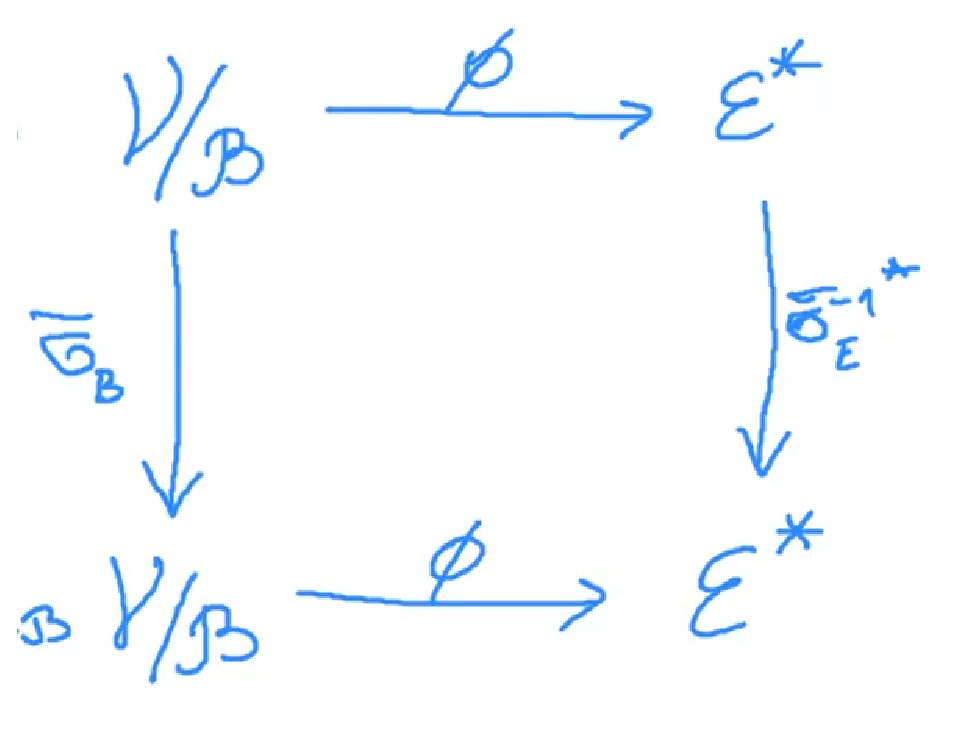
\includegraphics[scale=0.4]{seide_1.eps}
	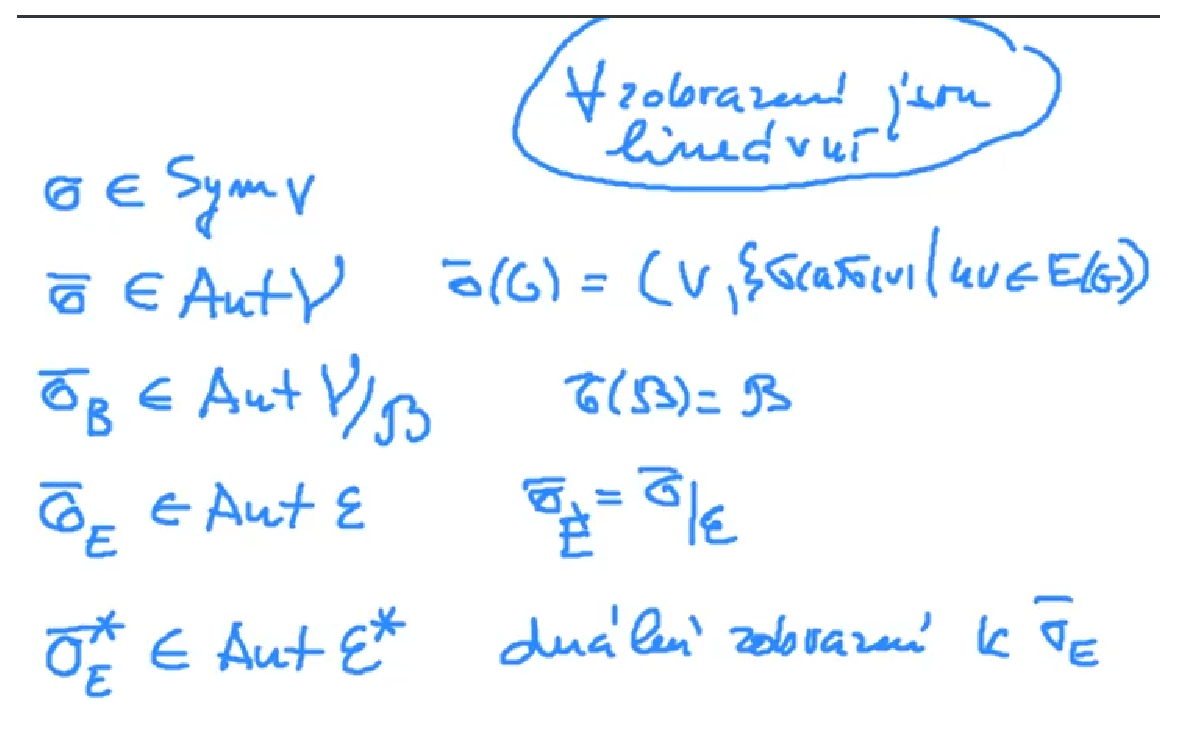
\includegraphics[scale=0.4]{seide_2.eps}

	Pak dle Burnsidova lemmatu: \# orbit $V/B$ pri akci $S(V) = \frac{1}{n!} \sum |(V/B)_{\sigma}|$.

	Taky \# orbit $\xi^{\ast}$ pri akci $S(V) = \frac{1}{n!} \sum |(\xi^{\ast})_{\sigma}| = \frac{1}{n!} \sum |(V/B)_{\sigma^{-1}}|$.
%todo
	Zbyva dokazat, ze \# orbit je stejny i pro $\xi$ misto $\xi^{\ast}$.

\end{proof}
